% Handbook figure snippets generated by scripts/export_handbook_mode_figures.py
% Paths are relative to the repository root.

\begin{figure}[htbp]
  \centering
  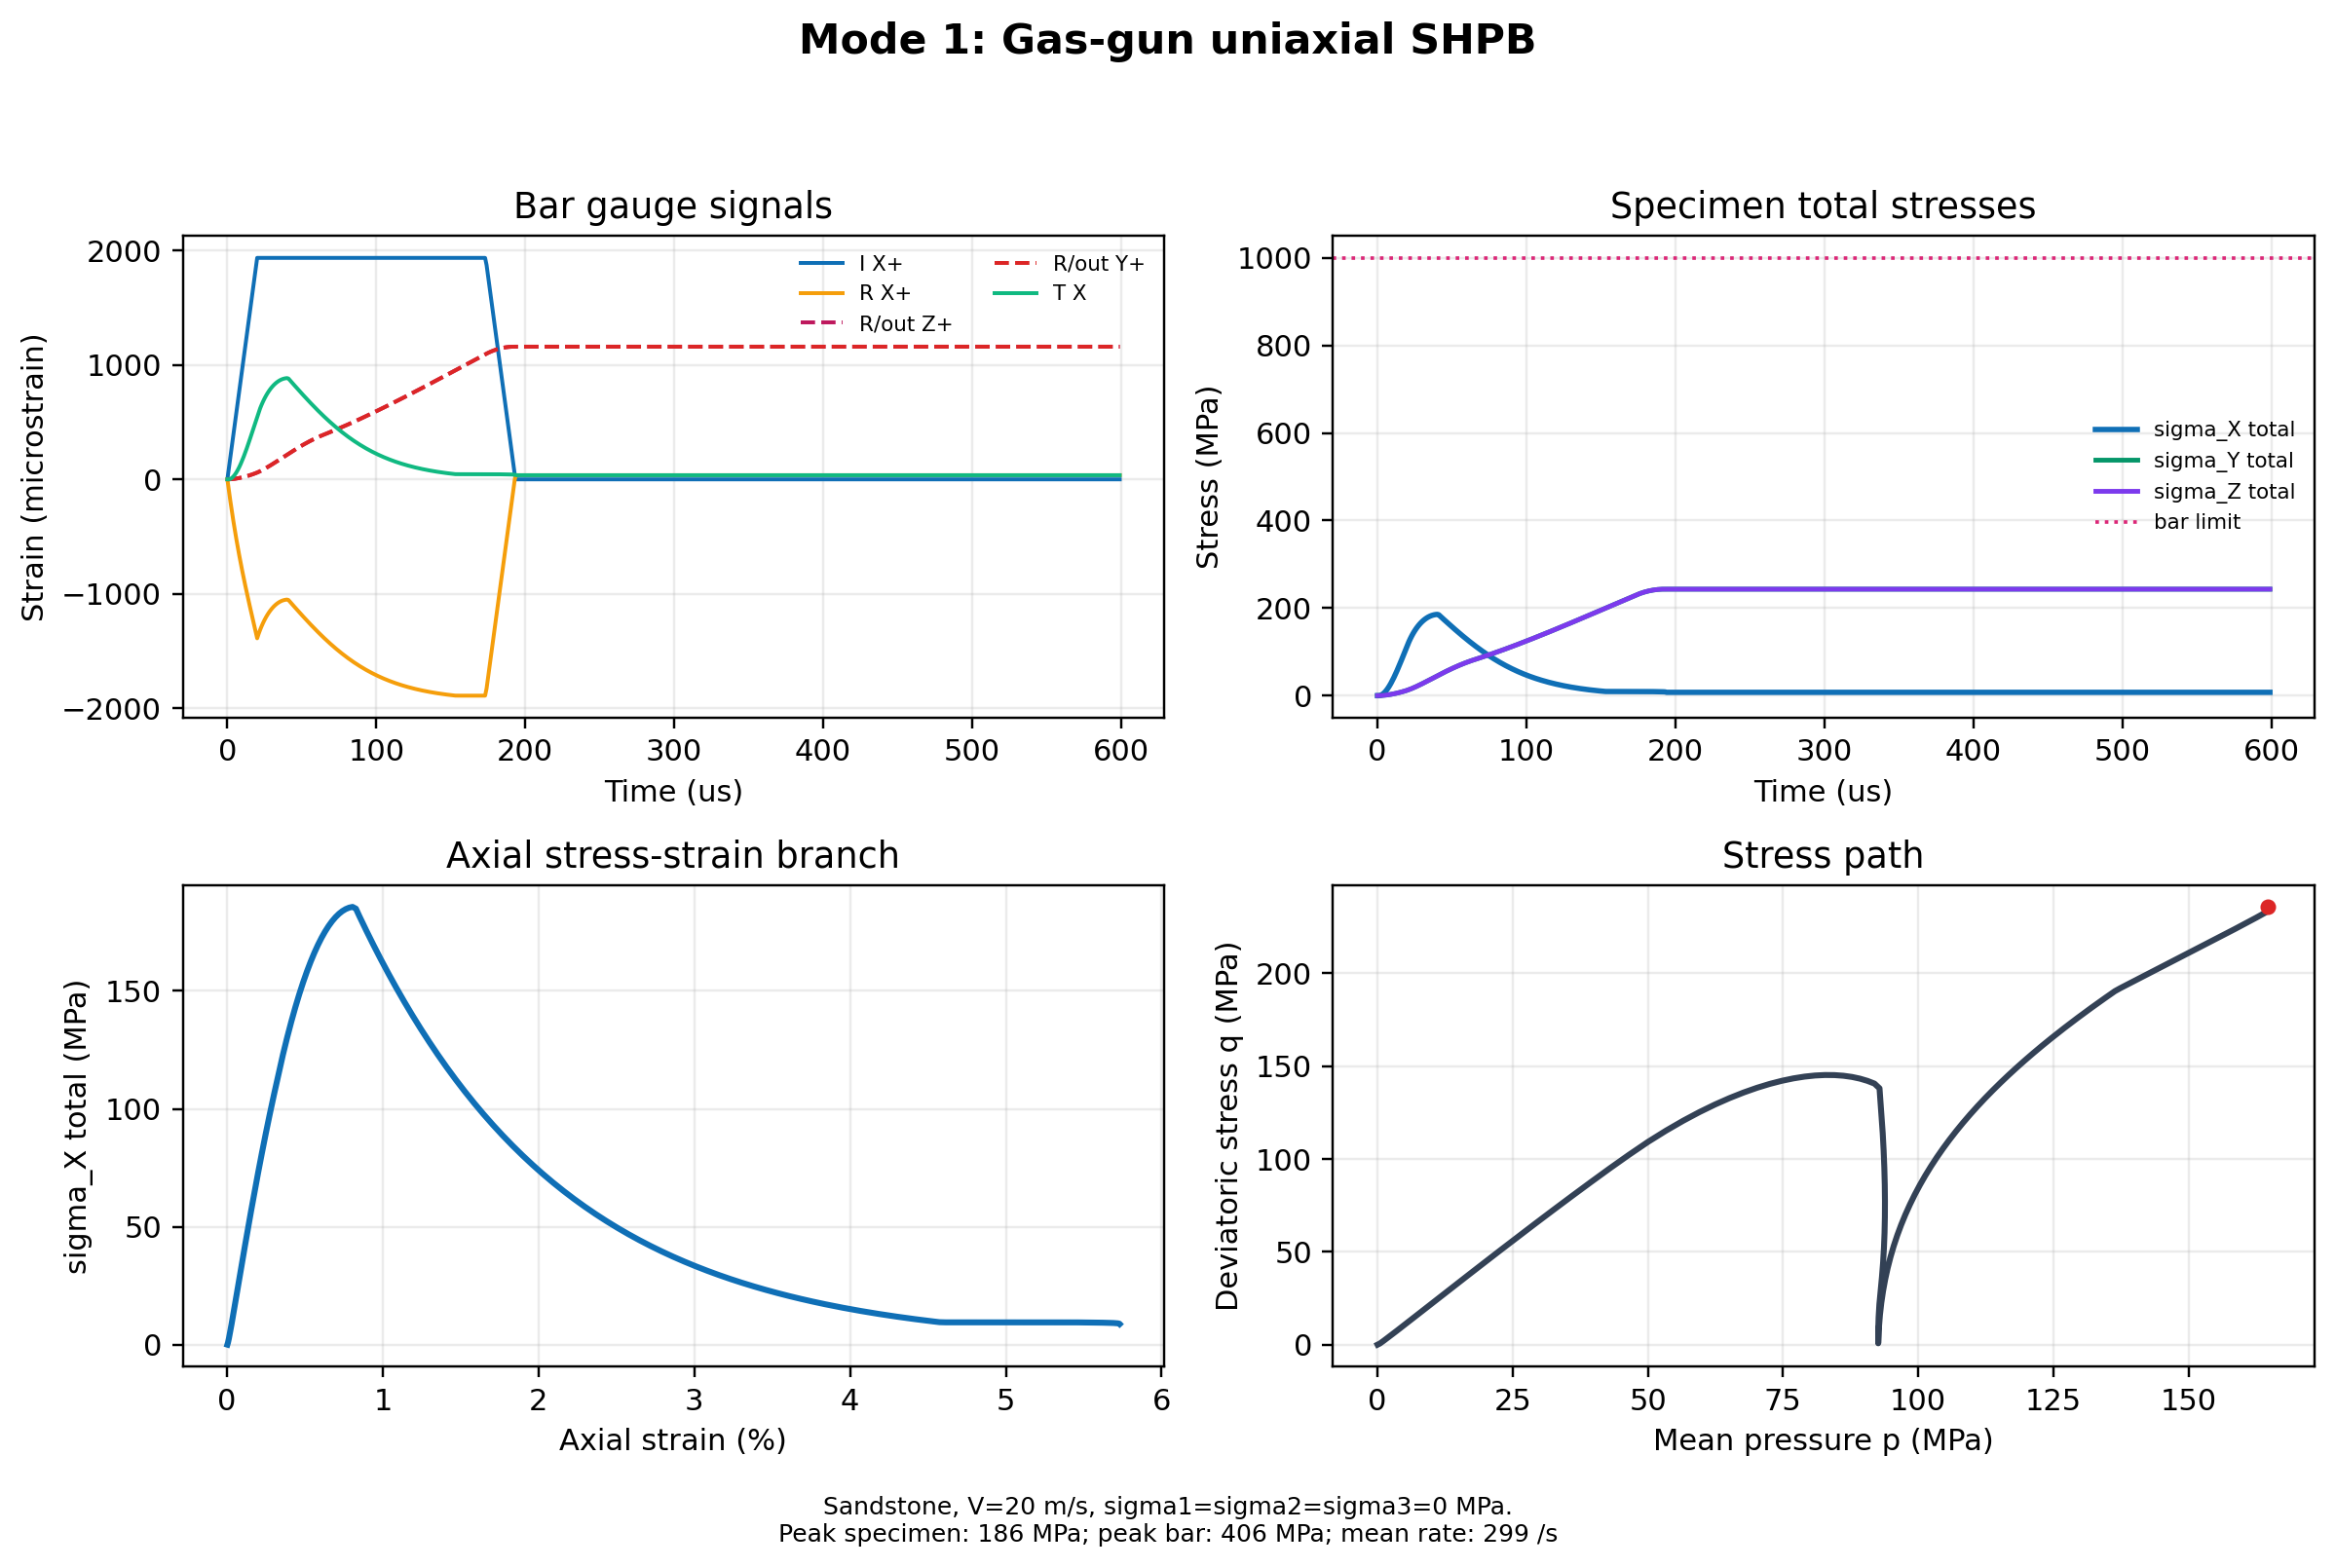
\includegraphics[width=\linewidth]{figures/handbook_modes/mode_1_gas_gun_uniaxial.png}
  \caption{Mode 1 sample run: sandstone, gas-gun uniaxial SHPB, V=20 m/s, no static confinement.}
  \label{fig:mode-1-gas-gun-uniaxial}
\end{figure}

\begin{figure}[htbp]
  \centering
  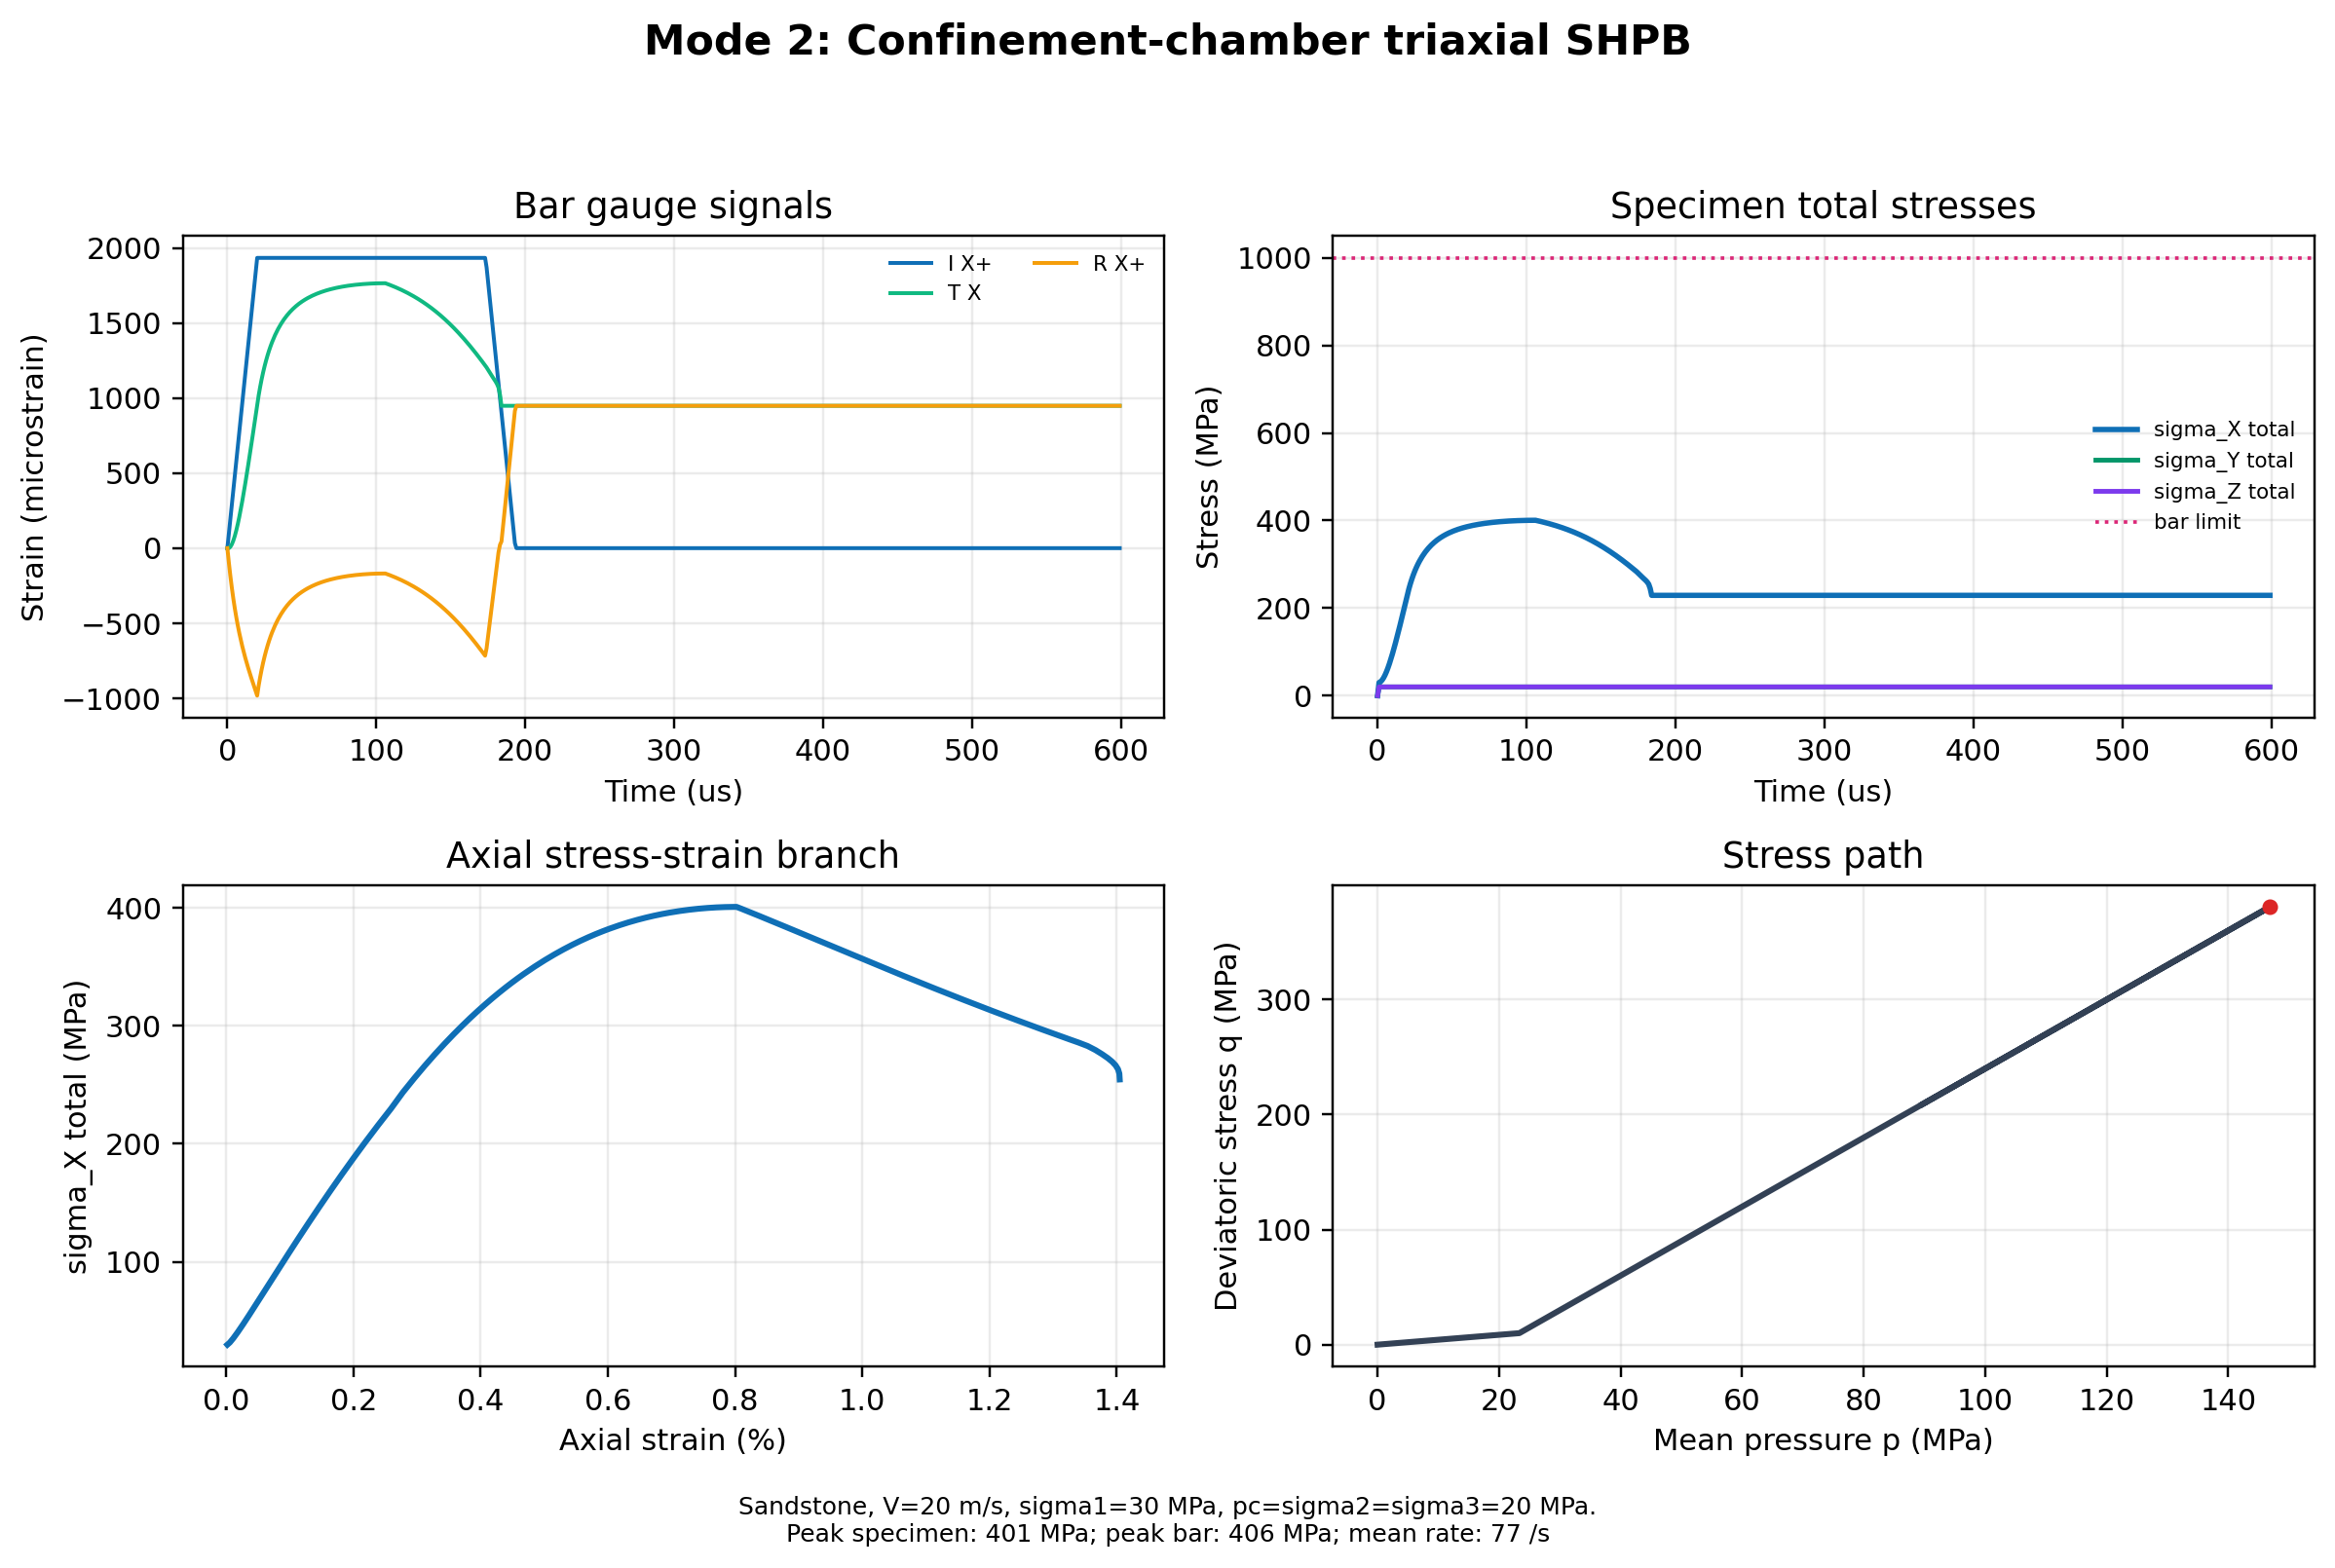
\includegraphics[width=\linewidth]{figures/handbook_modes/mode_2_confinement_chamber.png}
  \caption{Mode 2 sample run: sandstone in confinement chamber, V=20 m/s, sigma1=30 MPa and pc=20 MPa.}
  \label{fig:mode-2-confinement-chamber}
\end{figure}

\begin{figure}[htbp]
  \centering
  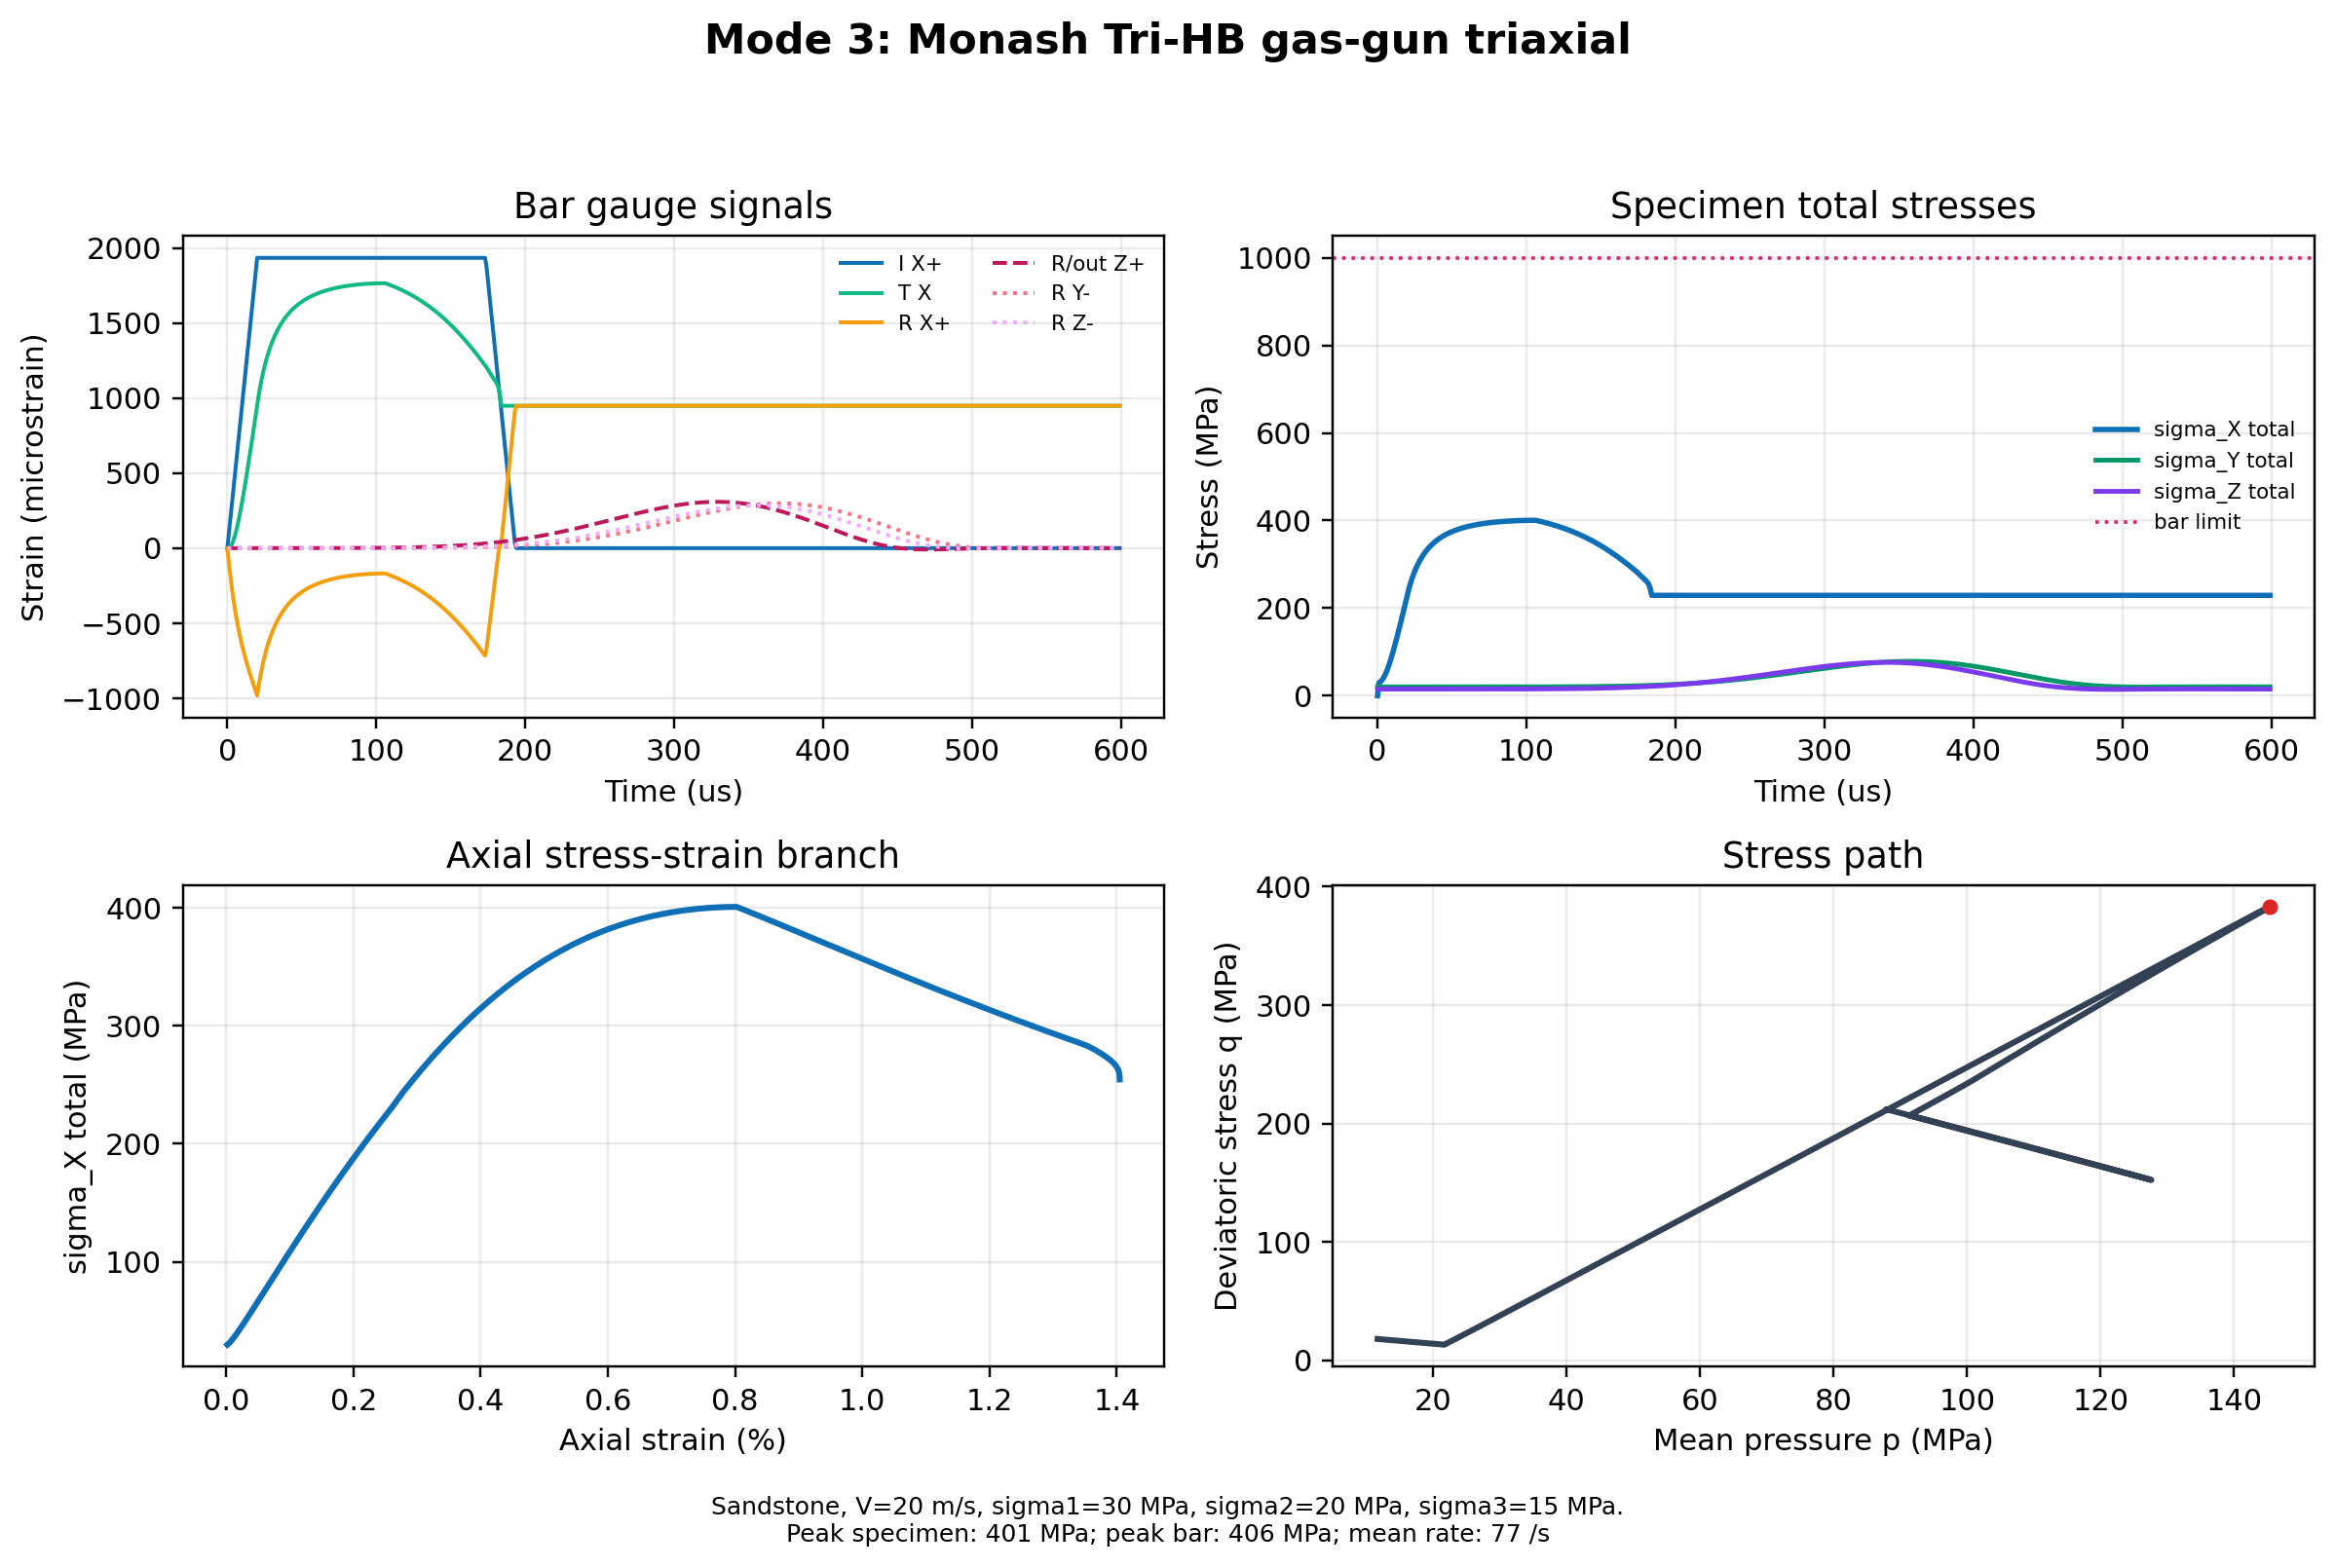
\includegraphics[width=\linewidth]{figures/handbook_modes/mode_3_monash_tri_hb.png}
  \caption{Mode 3 sample run: sandstone with independent static triaxial prestress, V=20 m/s.}
  \label{fig:mode-3-monash-tri-hb}
\end{figure}

\begin{figure}[htbp]
  \centering
  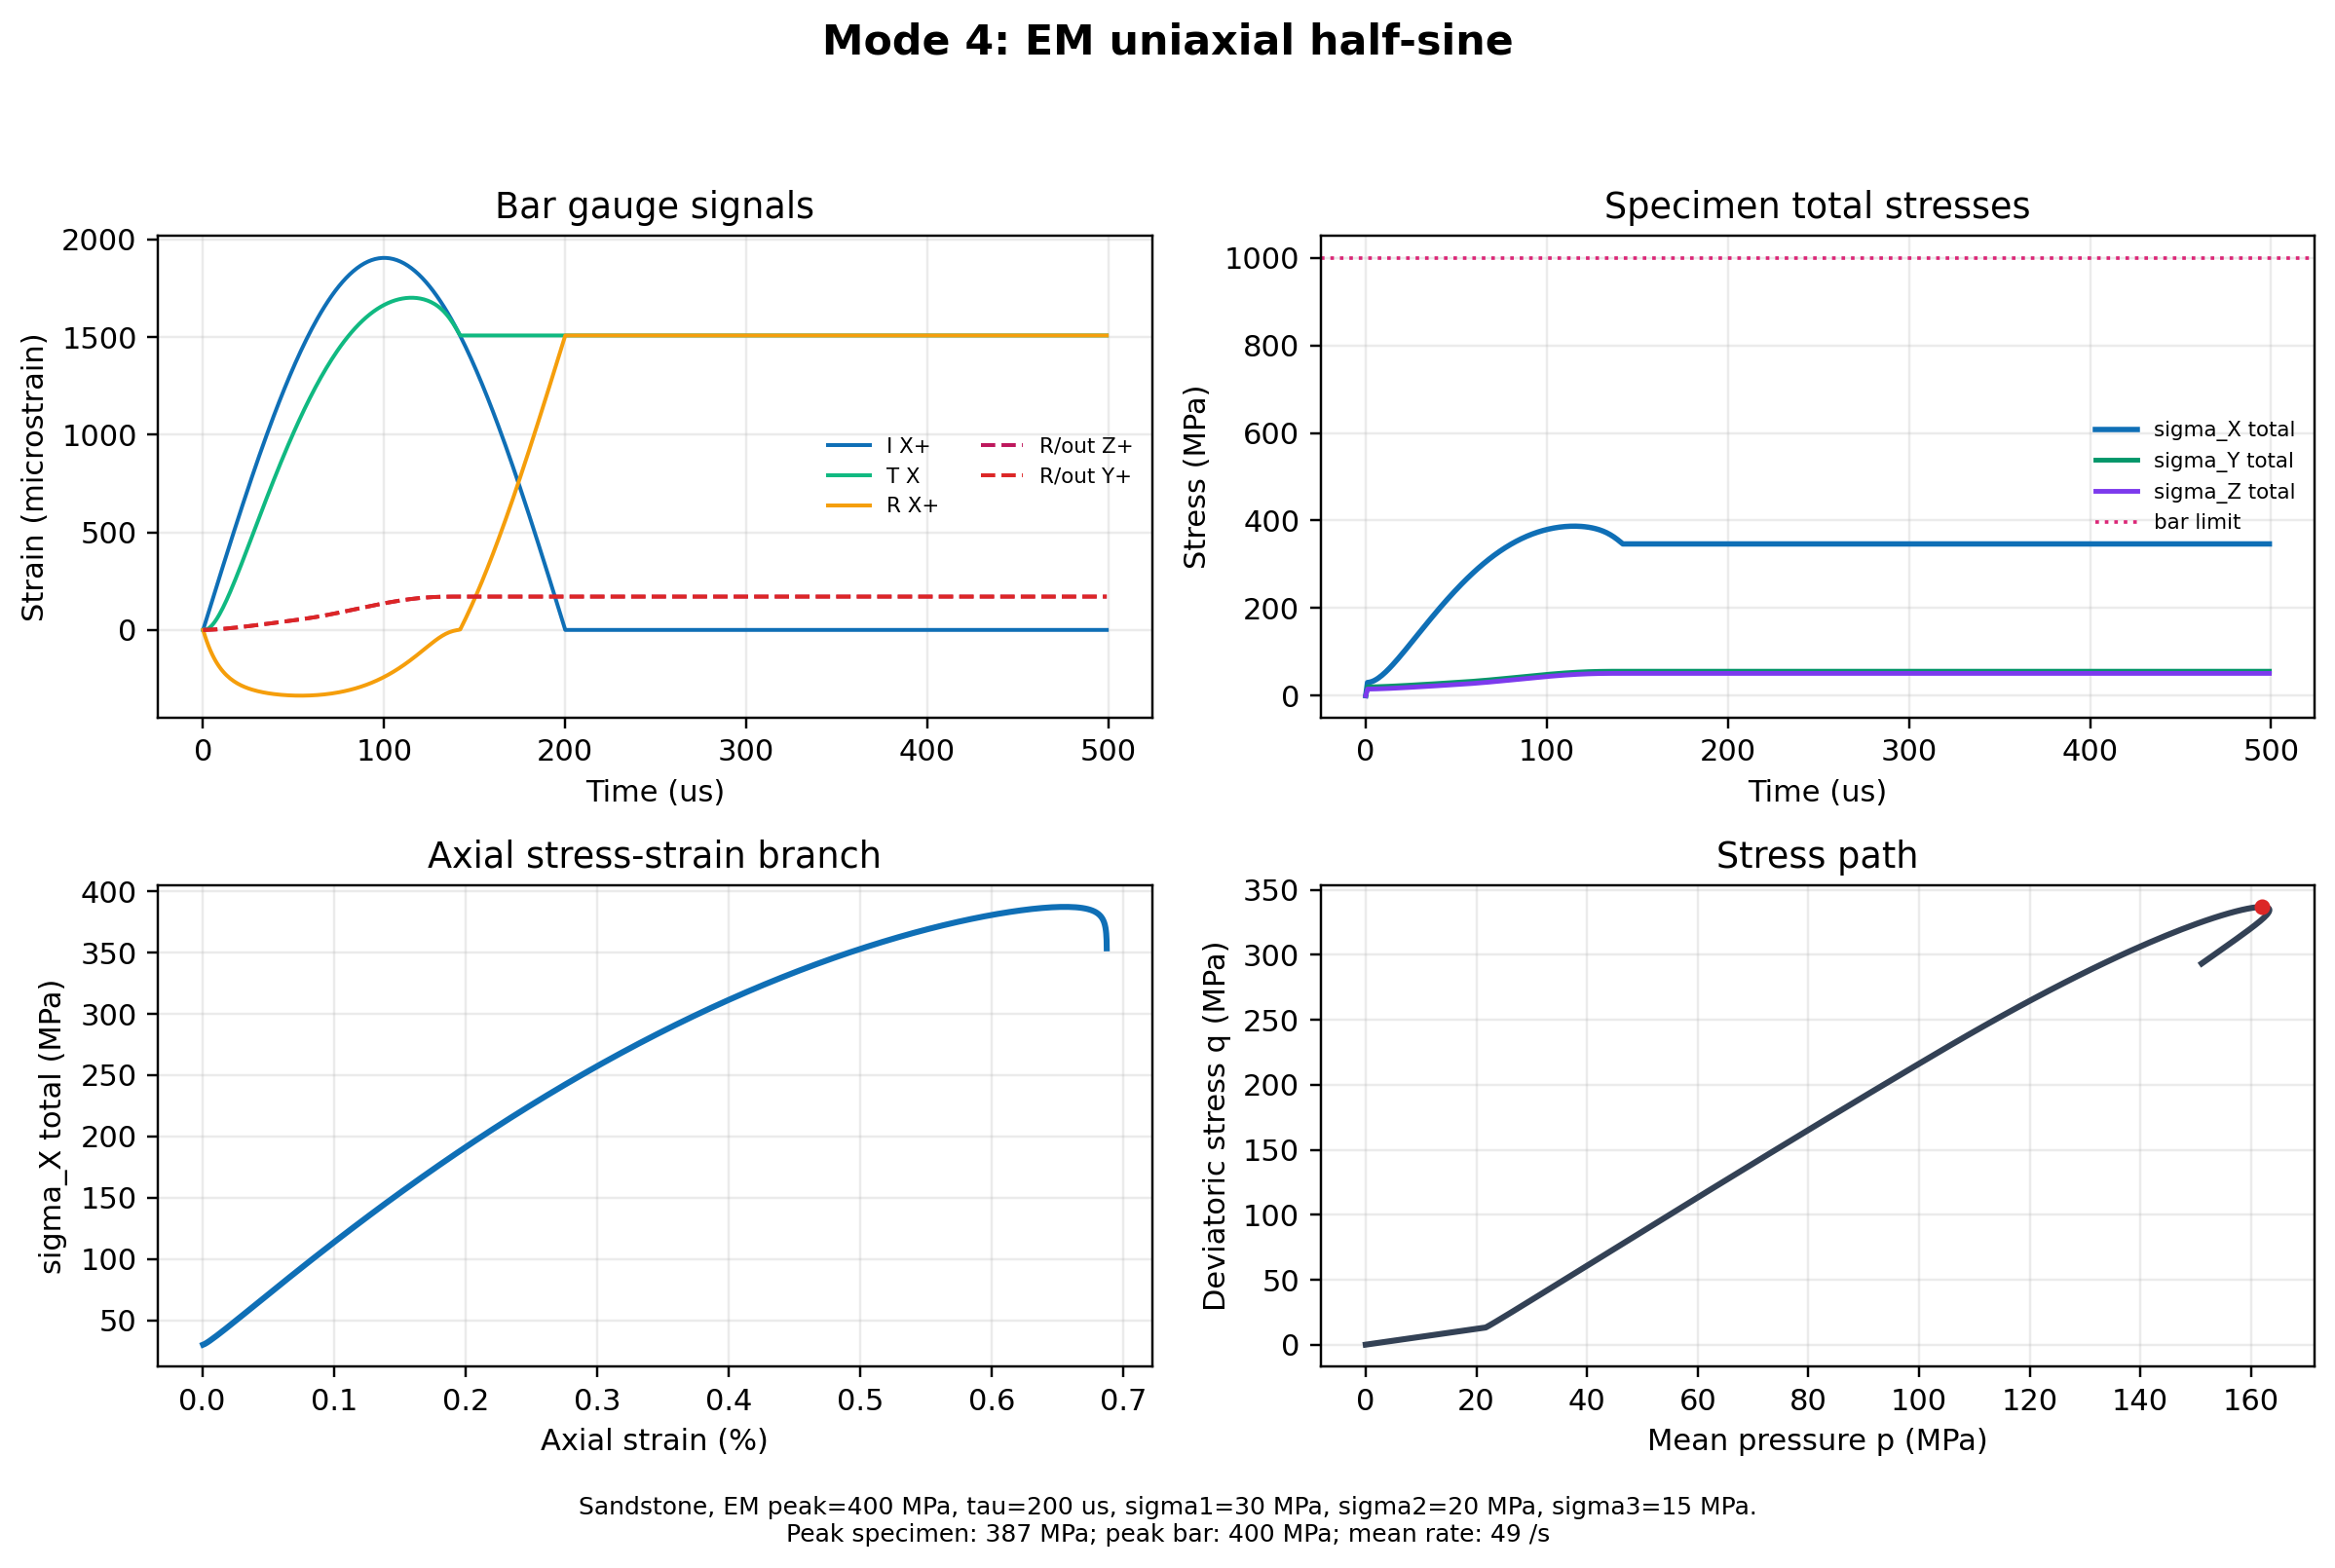
\includegraphics[width=\linewidth]{figures/handbook_modes/mode_4_em_uniaxial.png}
  \caption{Mode 4 sample run: sandstone, single EM half-sine pulse on +X, 400 MPa and 200 microseconds.}
  \label{fig:mode-4-em-uniaxial}
\end{figure}

\begin{figure}[htbp]
  \centering
  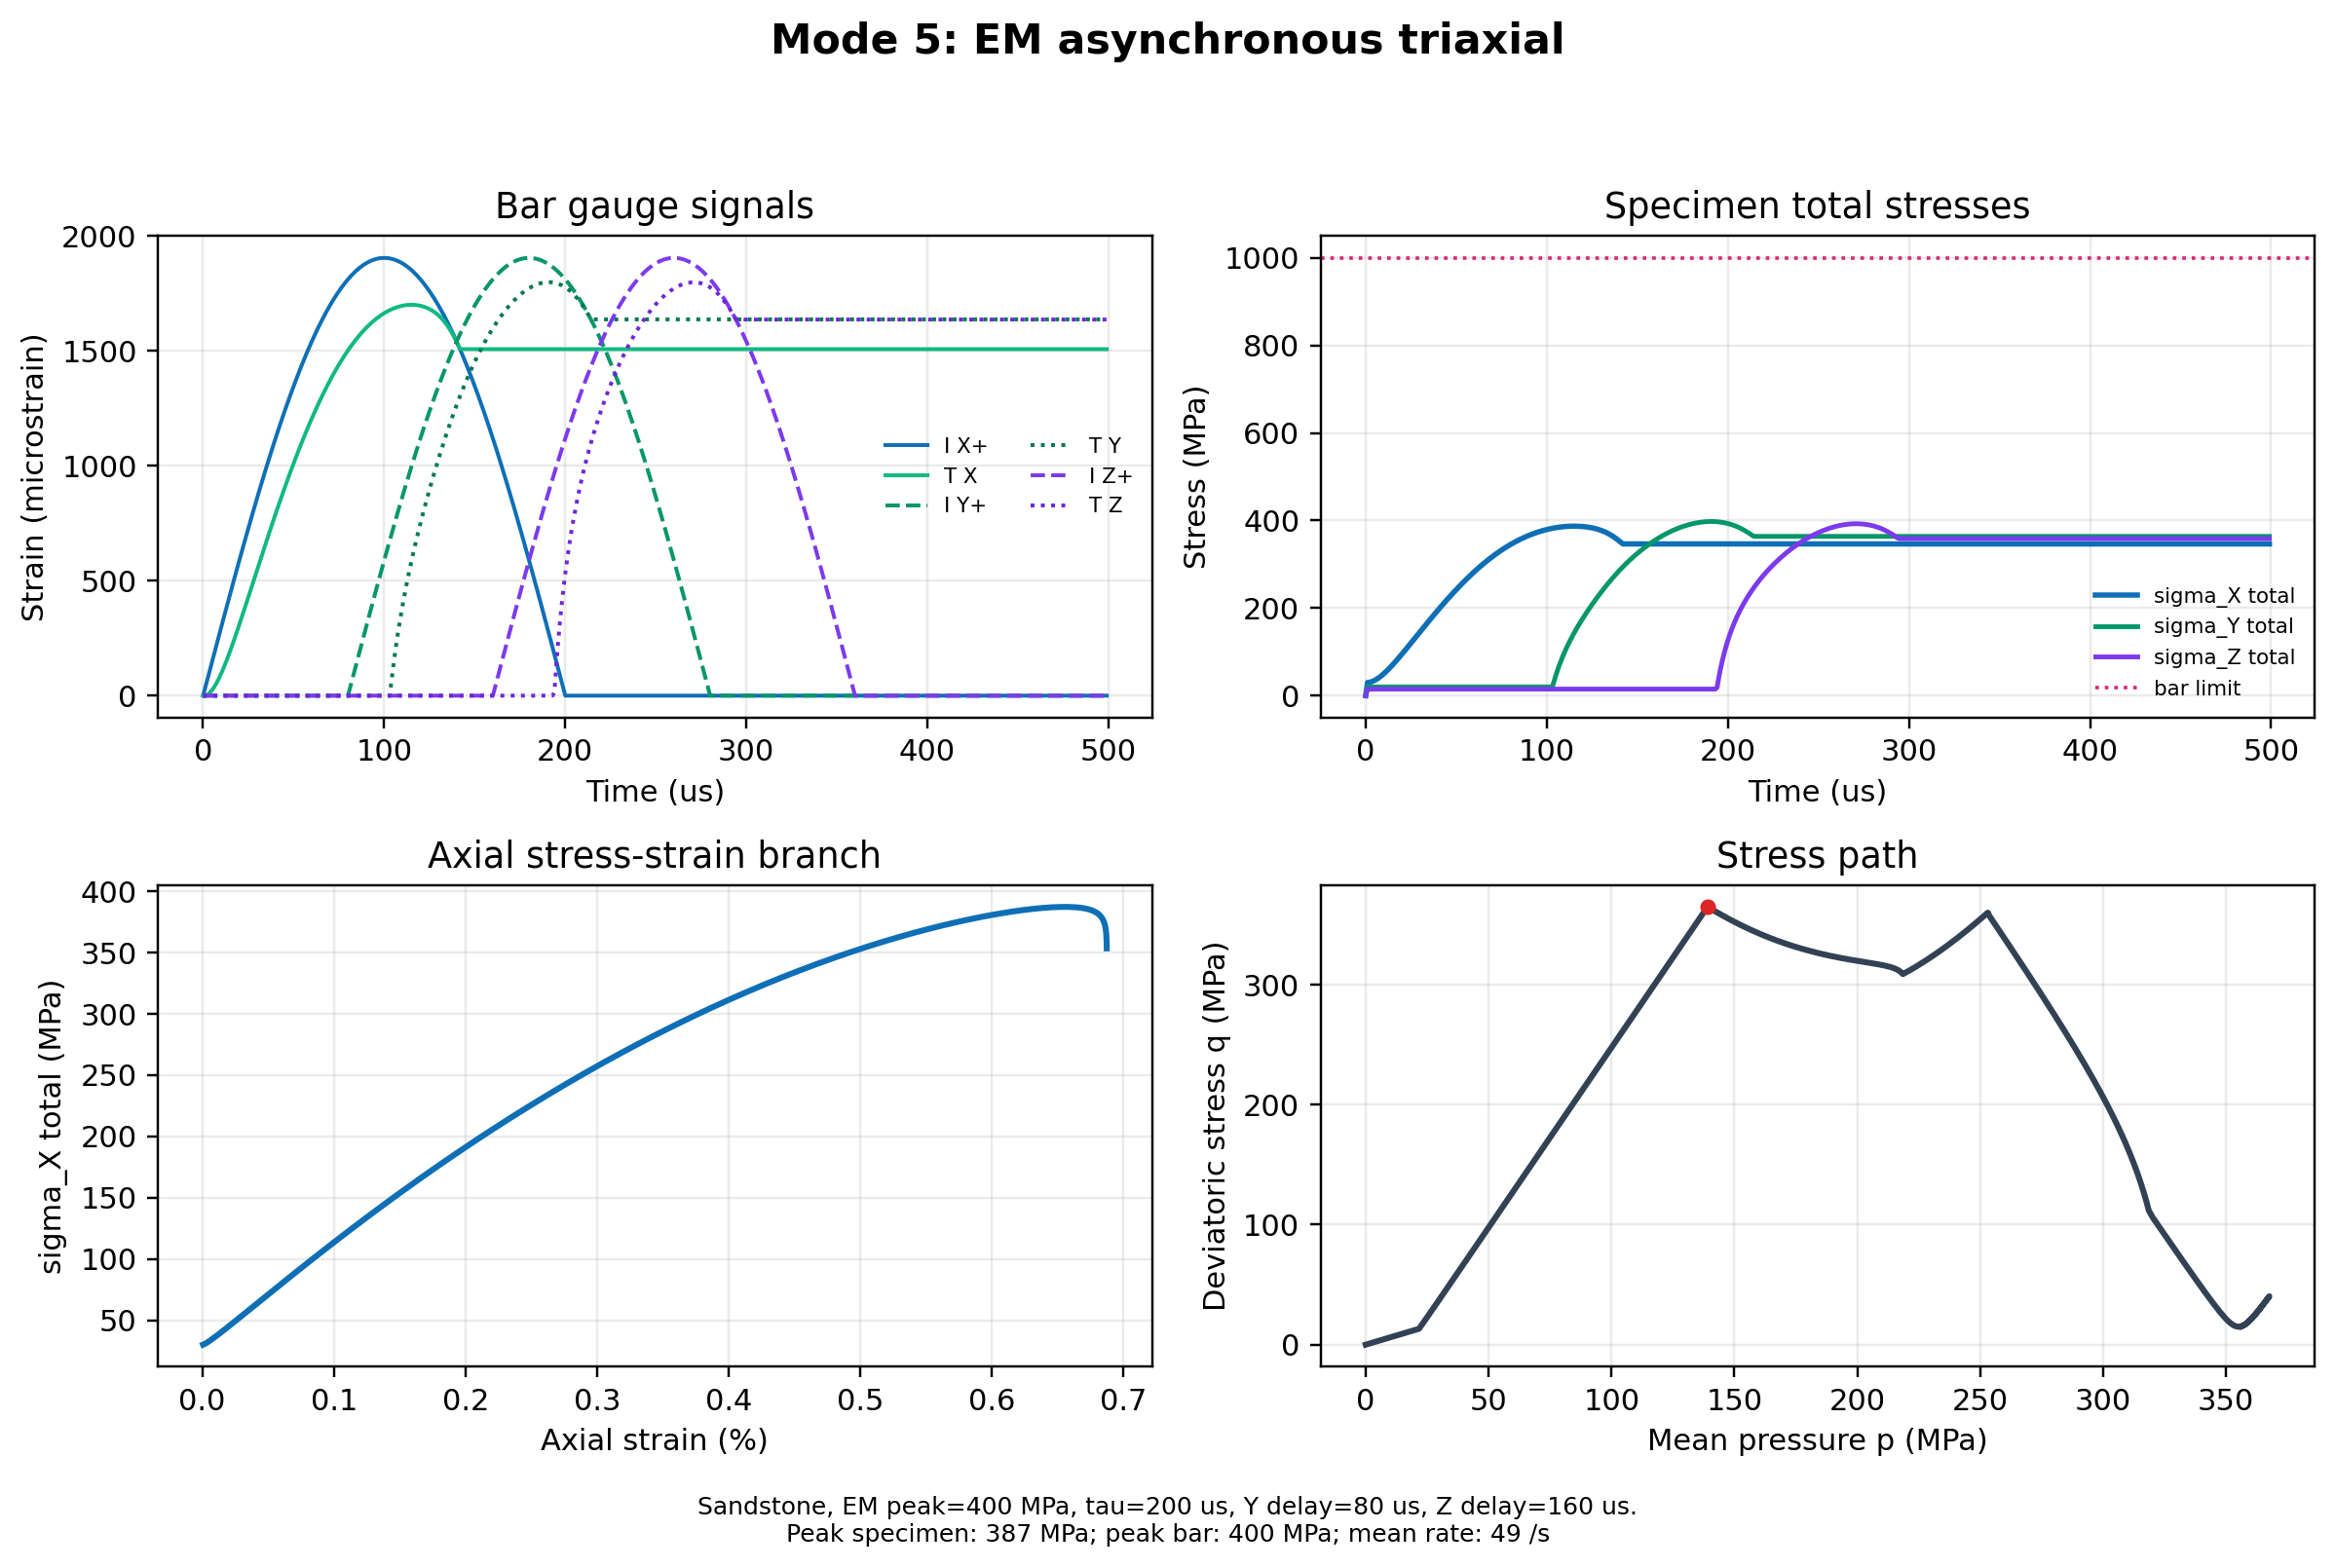
\includegraphics[width=\linewidth]{figures/handbook_modes/mode_5_em_async_triaxial.png}
  \caption{Mode 5 sample run: sandstone, EM pulses on +X, +Y, +Z with 80 and 160 microsecond delays.}
  \label{fig:mode-5-em-async-triaxial}
\end{figure}

\begin{figure}[htbp]
  \centering
  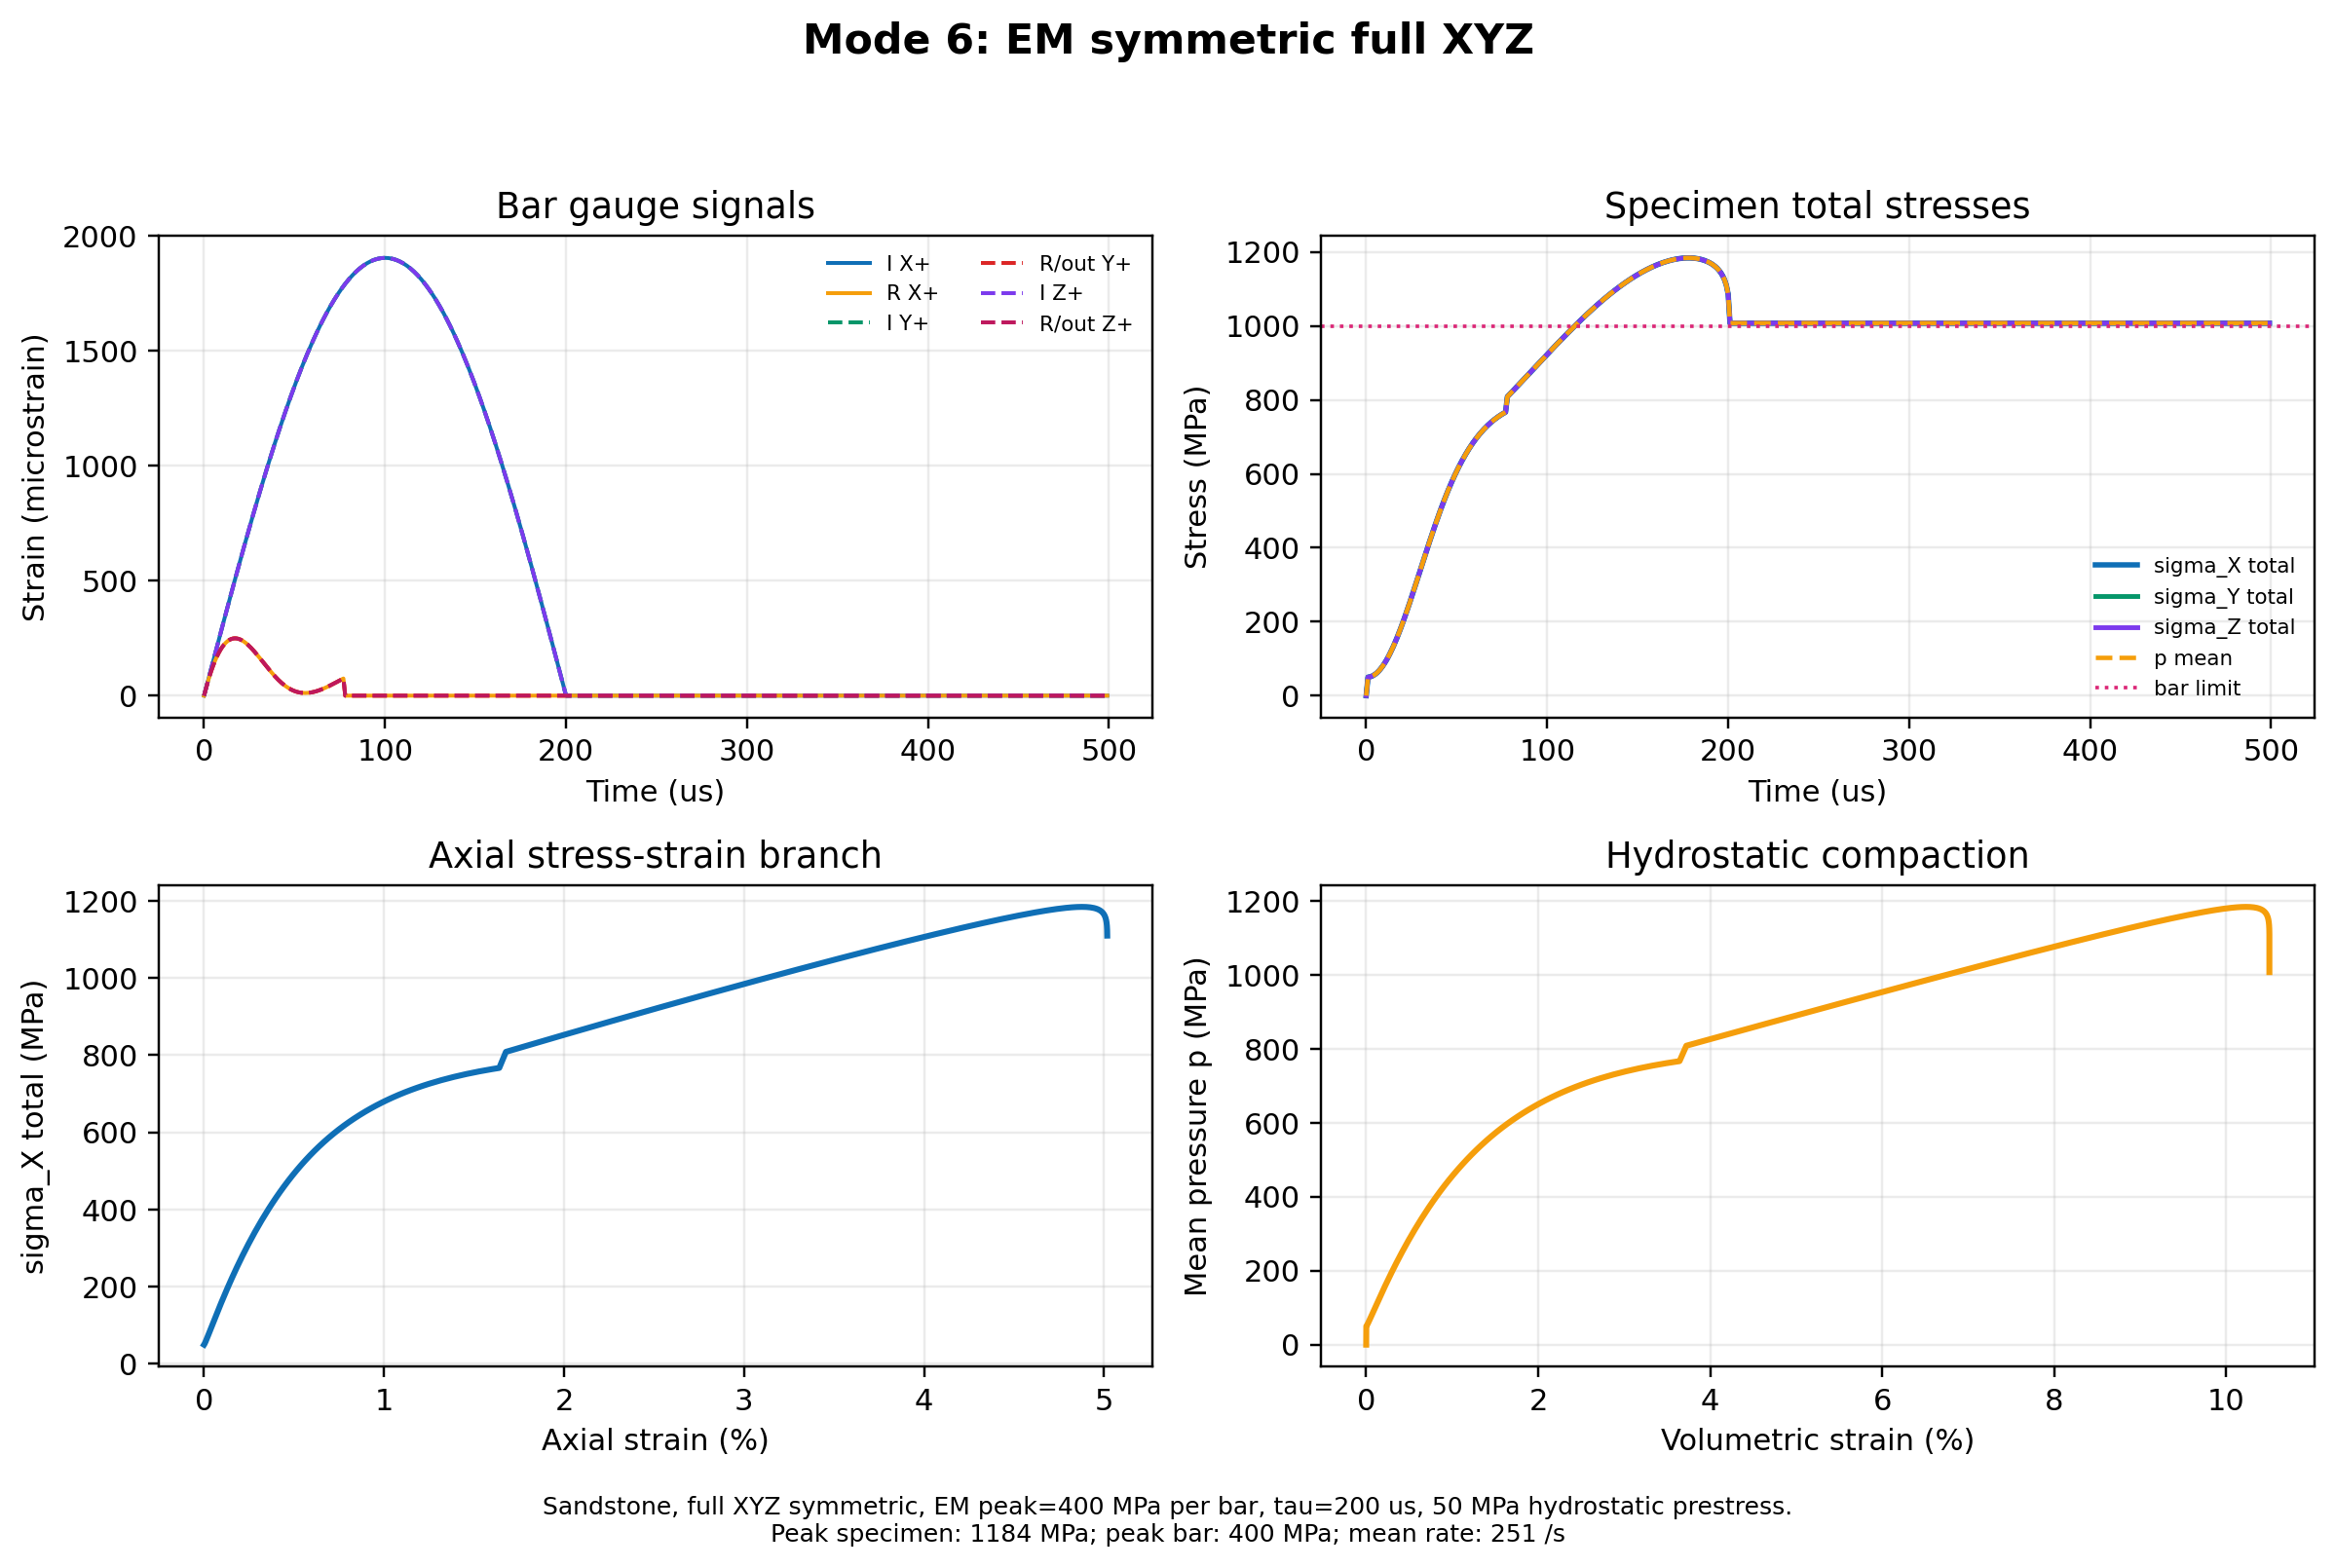
\includegraphics[width=\linewidth]{figures/handbook_modes/mode_6_em_symmetric_xyz.png}
  \caption{Mode 6 sample run: sandstone, full symmetric XYZ operation, 400 MPa single-bar pulse and 200 microseconds.}
  \label{fig:mode-6-em-symmetric-xyz}
\end{figure}
